\chapter{Результаты численного моделирования и сравнительный анализ}
\label{ch:results}

В данной главе представлены результаты анализа точности цилиндрической и конической аппроксимаций волновода, сравнение производительности реализованных численных решателей, а также результаты применения нейросетевых моделей для решения прямой и обратной задач волноводной акустики.

\section{Сравнение точности цилиндрической и конической аппроксимаций}
\label{sec:comparison_approx}

Для гладких геометрий (например, экспоненциального или катеноидального рупора) профиль площади поперечного сечения аппроксимируется набором дискретных элементов. Было проведено исследование сходимости решения при увеличении числа сегментов $N$ для цилиндрической и конической аппроксимаций.

В таблице~\ref{tab:errors} приведены значения среднеквадратичной ошибки (RMSE) для первых трех резонансных частот в зависимости от числа сегментов разбиения.

\begin{table}[h!]
    \centering
    \caption{Сравнение среднеквадратичной ошибки (RMSE, Гц) резонансных частот}
    \label{tab:errors}
    \begin{tabular}{|c|c|c|c|c|}
        \hline
        \multirow{2}{*}{Число сегментов $N$} & \multicolumn{2}{c|}{Цилиндрическая TMM} & \multicolumn{2}{c|}{Коническая TMM} \\
        \cline{2-5}
        & Резонанс 1 & Резонанс 2 & Резонанс 1 & Резонанс 2 \\
        \hline
        10  & 15.4 & 45.2 & 2.1  & 5.8  \\
        20  & 7.8  & 22.1 & 0.5  & 1.4  \\
        50  & 3.1  & 8.9  & 0.08 & 0.22 \\
        100 & 1.5  & 4.4  & 0.02 & 0.05 \\
        \hline
    \end{tabular}
\end{table}

Данные таблицы показывают, что коническая аппроксимация обеспечивает сходимость примерно на порядок быстрее по сравнению с цилиндрической при одинаковом числе сегментов $N$. Это объясняется более точным представлением производной площади $dA/dx$ в узлах сетки.

\section{Сравнение производительности решателей}
\label{sec:performance}

Проведено сравнение времени выполнения расчетов (в секундах) на стандартном наборе тестовых геометрий для Python-версии FDTD и C++ версии TLM. Результаты приведены в таблице~\ref{tab:performance}.

\begin{table}[h!]
    \centering
    \caption{Время выполнения расчета (в секундах) для 10000 временных шагов}
    \label{tab:performance}
    \begin{tabular}{|l|c|c|c|}
        \hline
        Метод & Язык реализации & Время работы (с) & Ускорение \\
        \hline
        FDTD (Webster) & Python & 2.45 & 1.0x \\
        TLM (Cylinder) & C++ & 0.08 & 30.6x \\
        \hline
    \end{tabular}
    \label{tab_count} % Для подсчета таблиц в аннотации
\end{table}

Использование C++ для реализации TLM-решателя позволило получить более чем 30-кратное ускорение расчетов во временной области, что критически важно для оптимизационных задач и обучения нейросетей на больших базах данных геометрий.

\section{Применение нейросетевого оператора (FNO)}
\label{sec:fno}

В качестве альтернативы традиционным численным решателям исследован подход на основе нейросетевого оператора Фурье (Fourier Neural Operator, FNO), обученного прогнозировать спектральный отклик (передаточную функцию $H_{\mathrm{dB}}(f)$) волновода по заданному дискретному профилю площадей сечений $\mathbf{a}$. 

В процессе валидации обученная модель FNO показала высокую точность аппроксимации: средняя абсолютная ошибка (MAE) по всему частотному диапазону составила $1.4299$ дБ, ошибка определения положения резонанса составила $11.1108$ дБ, а относительная ошибка по производной спектра --- $0.4680$ (подробные результаты приведены в табл.~\ref{tab:modifications_comparison} в главе~\ref{ch:direct_problem}). 

Благодаря параллельным тензорным вычислениям, время инференса FNO-модели на одном объекте составляет менее $1$ мс, что обеспечивает ускорение расчетов на несколько порядков по сравнению с классическими численными решателями на плотных сетках и делает данный подход перспективным для акустического моделирования в задачах реального времени.

\section{Решение обратной задачи восстановления геометрии}
\label{sec:inverse_problem}

Обратная задача волноводной акустики заключается в восстановлении продольного профиля площади поперечного сечения $A(x)$ волновода по заданной передаточной функции $H(f)$ (АЧХ). Данная задача является некорректно поставленной по Адамару из-за нелинейности отображения, а также физической неединственности решения (несколько существенно различающихся геометрий могут иметь крайне близкие спектральные отклики).

В рамках данной работы были исследованы два принципиально разных класса методов решения обратной задачи:
\begin{enumerate}
    \item Оптимизационные методы в пространстве параметров (градиентный спуск с обратным распространением ошибки через дифференцируемый нейросетевой эмулятор и стохастический поиск методом Метрополиса --- MCMC).
    \item Нейросетевой подход, основанный на обучении сверточной архитектуры типа UNet для прямого отображения спектральной карты в геометрический профиль.
\end{enumerate}

\subsection{Оптимизационные методы: градиентный спуск и метод Метрополиса}
\label{subsec:opt_methods}

В первом подходе обратная задача формулируется как минимизация невязки между целевой АЧХ $H_{\mathrm{target}}(f)$ и откликом текущей геометрии $\mathcal{F}_{\theta}(\mathbf{a})$, вычисляемым с помощью обученного нейросетевого оператора. Минимизация проводилась двумя способами:
\begin{itemize}
    \item \textbf{Градиентный спуск}: нахождение градиентов целевой функции невязки по входным площадям сечений $\mathbf{a}$ с помощью автоматического дифференцирования в PyTorch и оптимизация методом Adam.
    \item \textbf{Метод Метрополиса (МСМС)}: случайный блуждающий поиск в пространстве площадей с вероятностью принятия шага, пропорциональной уменьшению невязки АЧХ.
\end{itemize}

Результаты восстановления тестового профиля волновода обоими методами представлены на рис.~\ref{fig:inverse_opt_comparison}.

\begin{figure}[H]
    \centering
    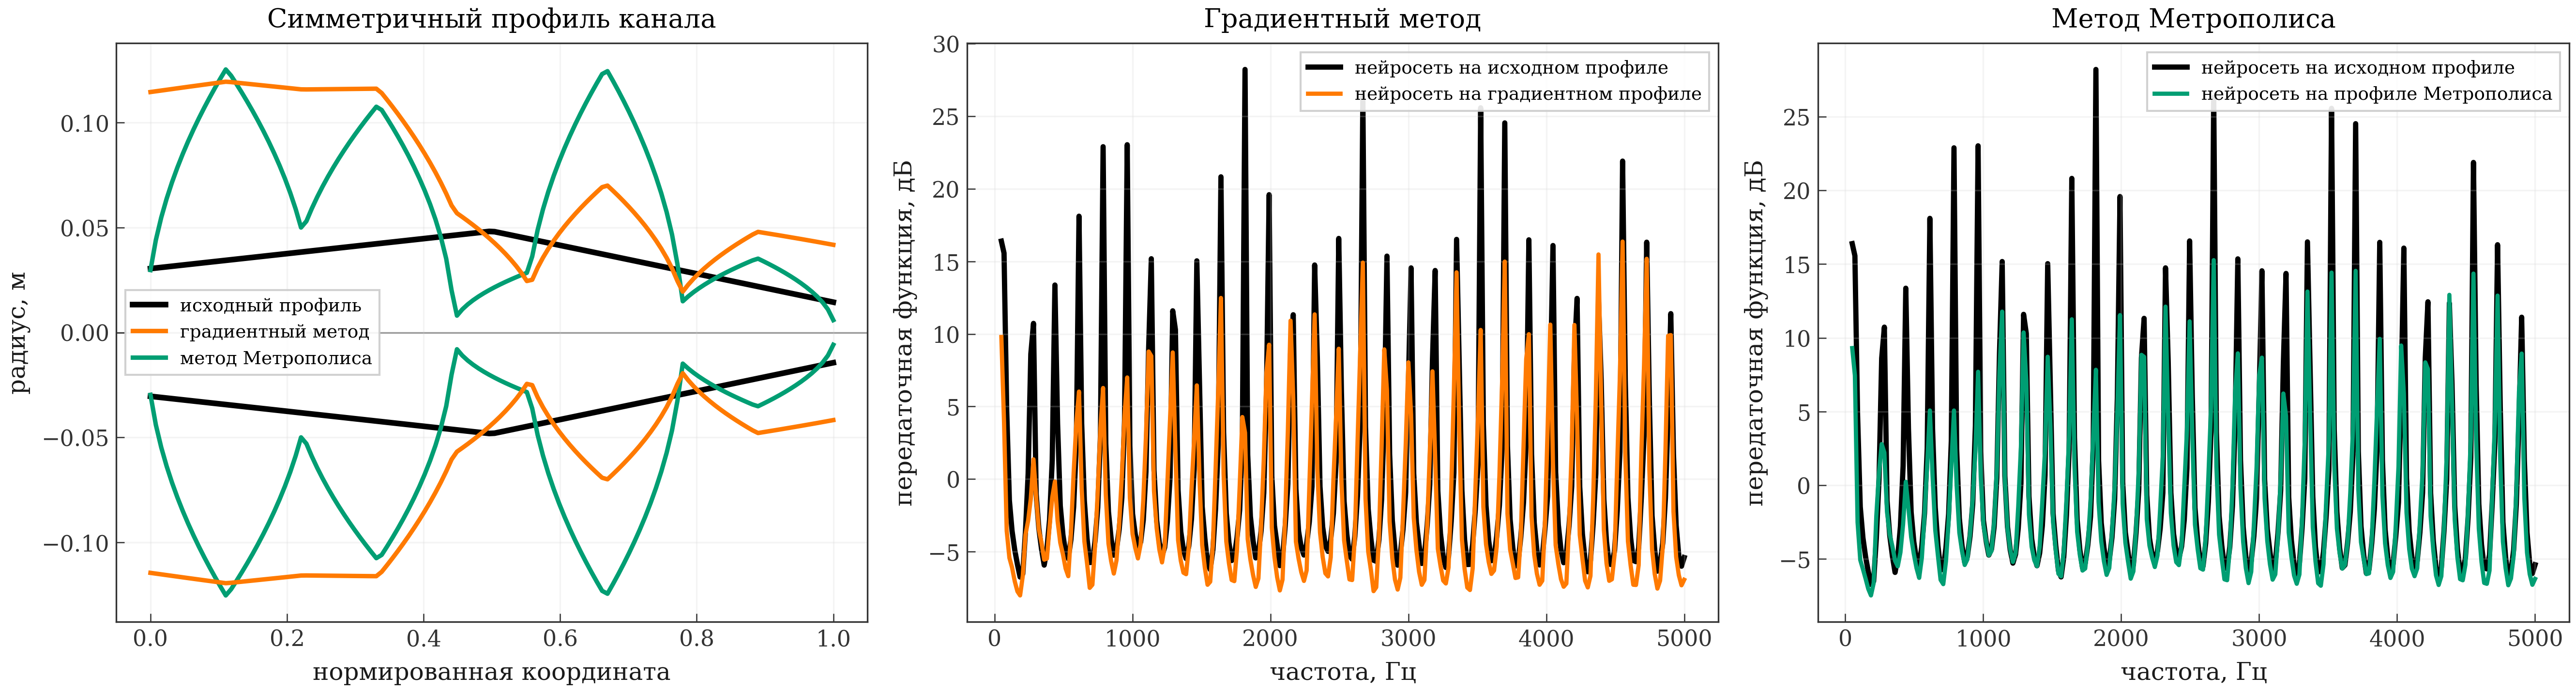
\includegraphics[width=0.95\textwidth]{images/обратная_задача_сравнение_методов.png}
    \caption{Сравнение результатов восстановления геометрии волновода и соответствующих АЧХ с помощью градиентного спуска и метода Метрополиса.}
    \label{fig:inverse_opt_comparison}
\end{figure}

Как видно из графиков геометрии (слева на рис.~\ref{fig:inverse_opt_comparison}), оба метода предсказывают довольно плохую форму исходного канала (наблюдаются сильные отклонения от истинного профиля площадей), что подтверждает неединственность решения обратной задачи. Однако при анализе соответствующих АЧХ (справа на рис.~\ref{fig:inverse_opt_comparison}) видно, что метод Метрополиса обеспечивает значительно более точную аппроксимацию спектрального отклика. В частности, метод Метрополиса дает более или менее правильные нижние границы $H$ (положение и глубину провалов АЧХ), тогда как градиентный спуск застревает в локальных минимумах и не может восстановить антирезонансы.

\subsection{Глубокое обучение: UNet на картах [H, f, x]}
\label{subsec:unet_inverse}

Для преодоления ограничений традиционной оптимизации был разработан метод на основе сверточной нейросети UNet (\text{TransferMapInverseUNet}). Поскольку стандартный спектральный отклик является одномерным вектором $H(f) \in \mathbb{R}^{N_f}$, а геометрия имеет пространственную размерность $A(x) \in \mathbb{R}^{N_s}$, для применения 2D-сверток одномерная АЧХ преобразуется в 2D пространственно-спектральную карту входа размерности $[C, N_f, N_s]$.

Были исследованы два режима формирования входной карты (рис.~\ref{fig:unet_input_map}):
\begin{itemize}
    \item \textbf{Режим трансляции (Broadcast)}: одномерная целевая АЧХ дублируется вдоль всей пространственной оси $x$, формируя однородную сетку.
    \item \textbf{Режим префиксного решателя (Prefix Solver)}: каждый столбец $j$ входной карты содержит АЧХ усеченной геометрии $[0, x_j]$, что позволяет физически связать частотный отклик с координатой распространения волны.
\end{itemize}

Входной тензор имеет три канала ($C=3$), содержащих значения АЧХ $H_{\mathrm{dB}}(f)$, нормированные частоты $f$ и нормированные пространственные координаты $x$.

\begin{figure}[H]
    \centering
    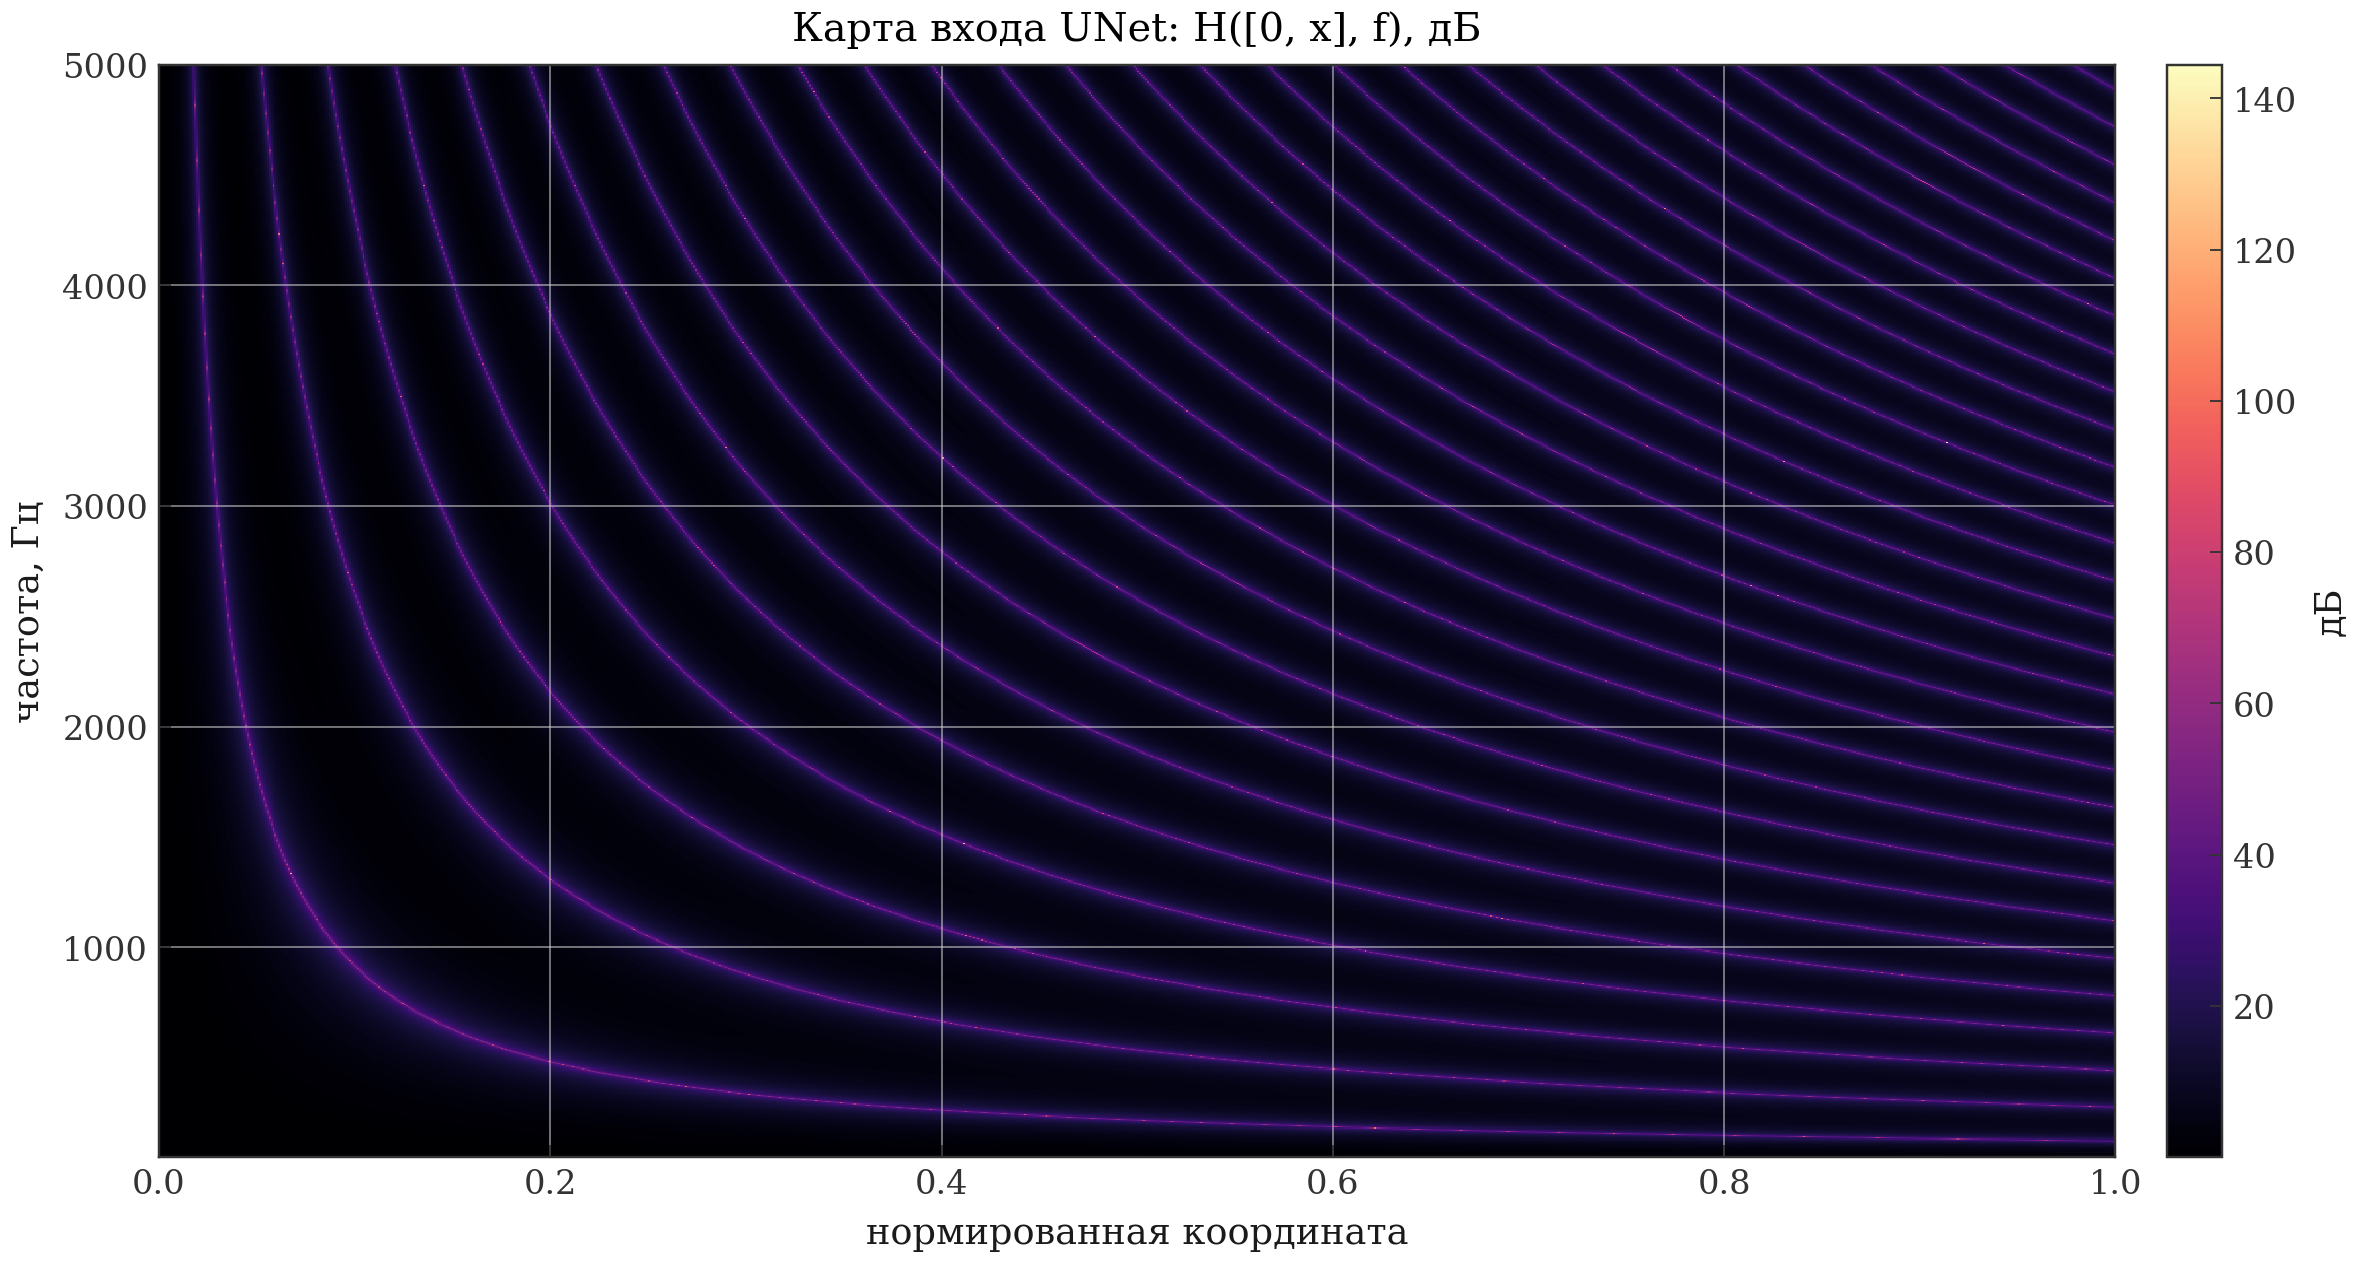
\includegraphics[width=0.85\textwidth]{images/обратная_задача_суперкарта.png}
    \caption{Пример двумерной входной пространственно-спектральной карты $[H, f, x]$ (суперкарты) высокого разрешения для сверточной модели UNet.}
    \label{fig:unet_input_map}
\end{figure}

Сверточная модель UNet обучается предсказывать 1D геометрический профиль волновода $A(x)$ по 2D входной карте. На рис.~\ref{fig:unet_input_maps_four} представлены двумерные входные пространственно-спектральные карты для четырех тестовых образцов волноводов, а результаты восстановления площадей сечений для них показаны на рис.~\ref{fig:unet_reconstructions}.

\begin{figure}[H]
    \centering
    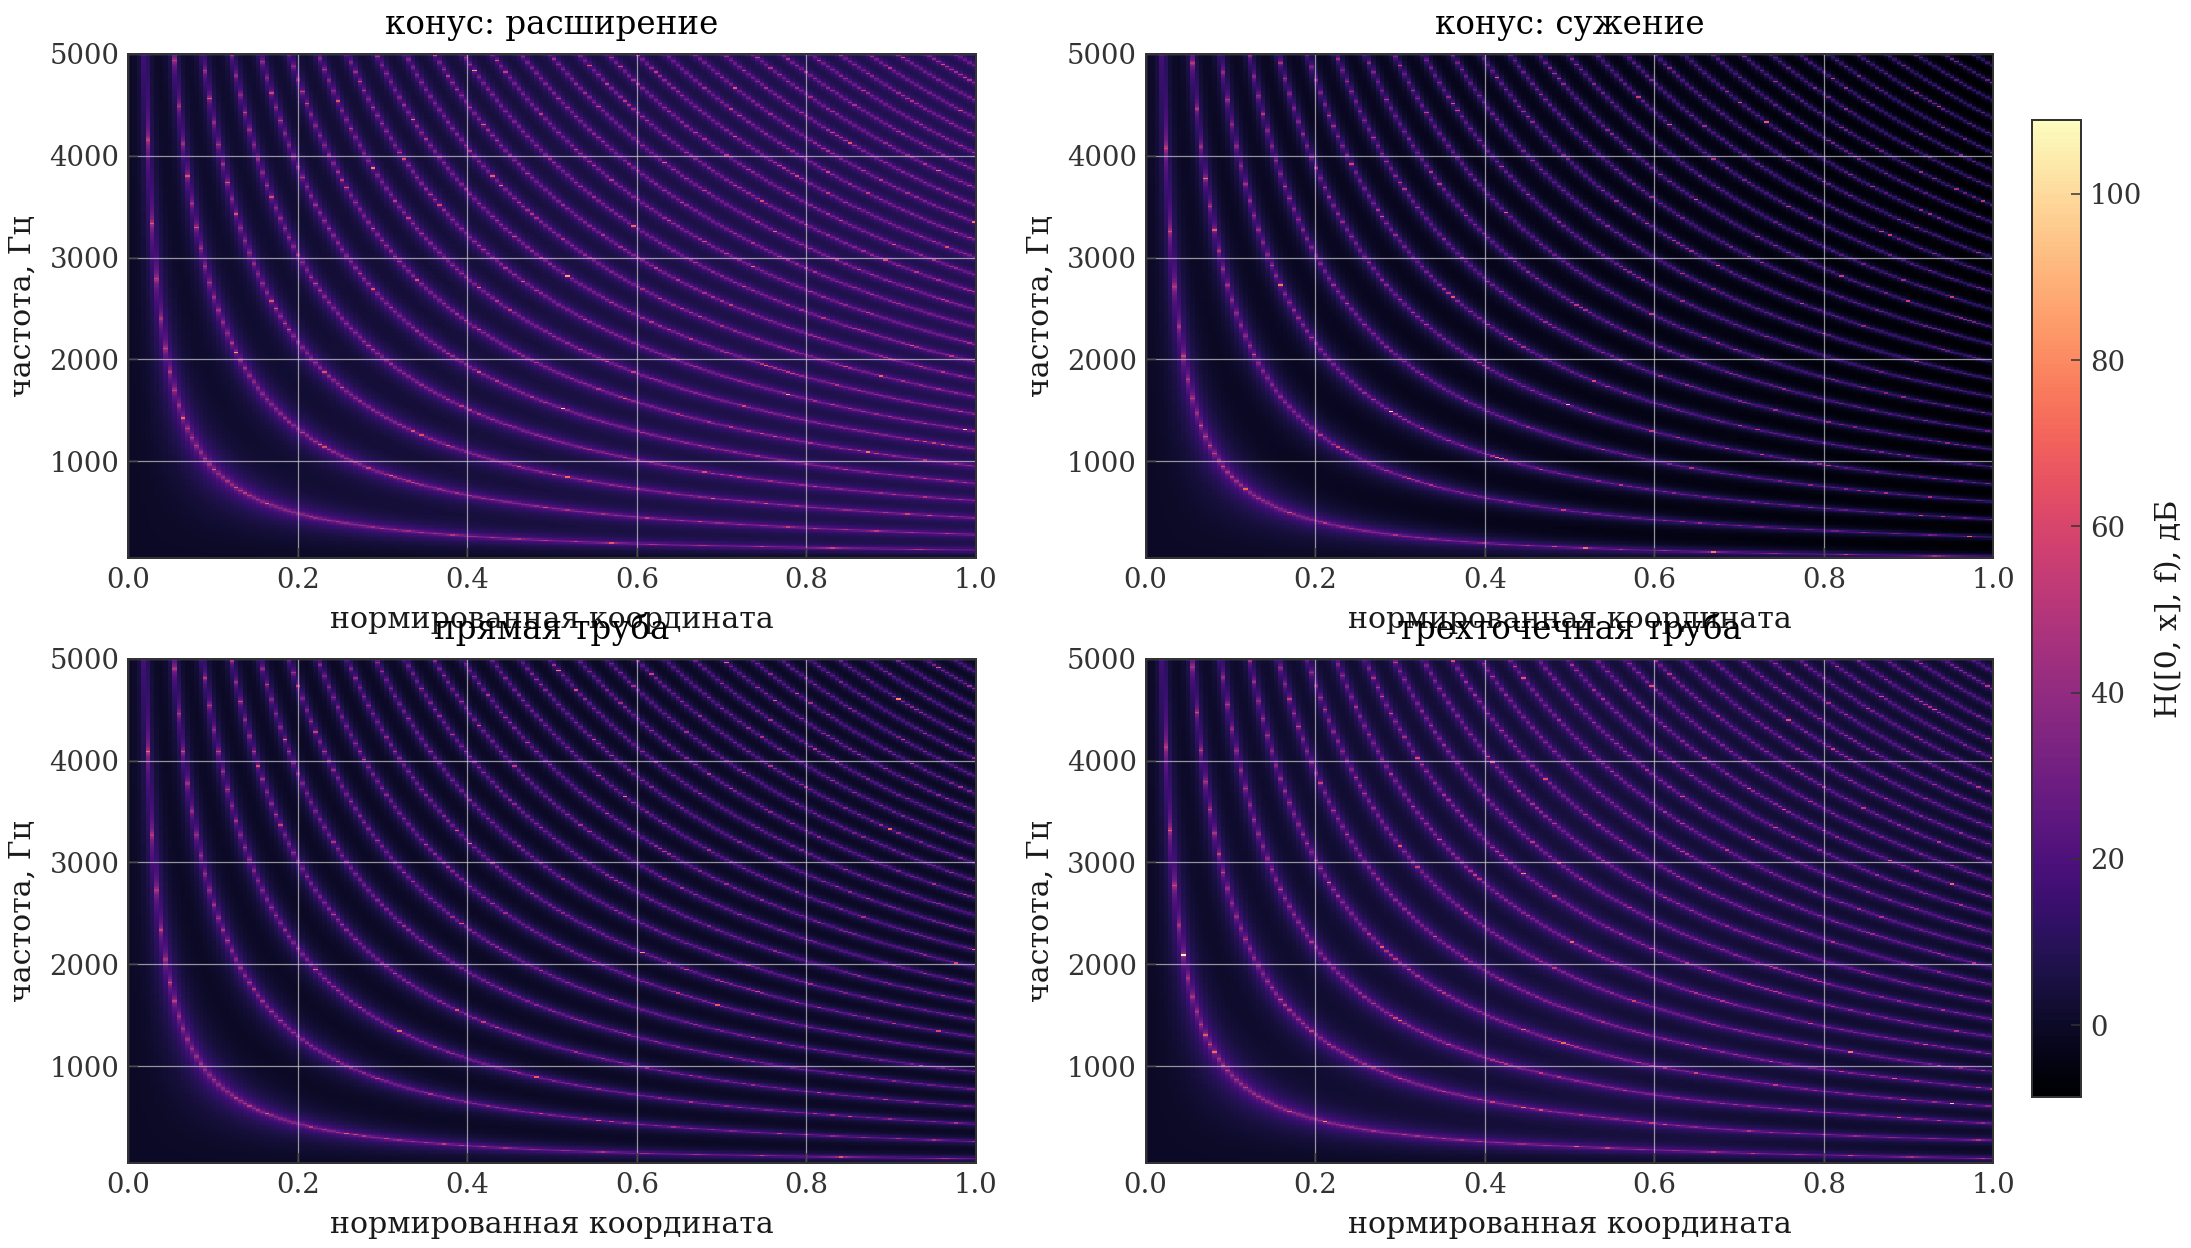
\includegraphics[width=0.95\textwidth]{images/обратная_задача_карты_к_трубам.png}
    \caption{Двумерные входные карты $[H, f, x]$ для четырех тестовых волноводов, используемые моделью UNet.}
    \label{fig:unet_input_maps_four}
\end{figure}

\begin{figure}[H]
    \centering
    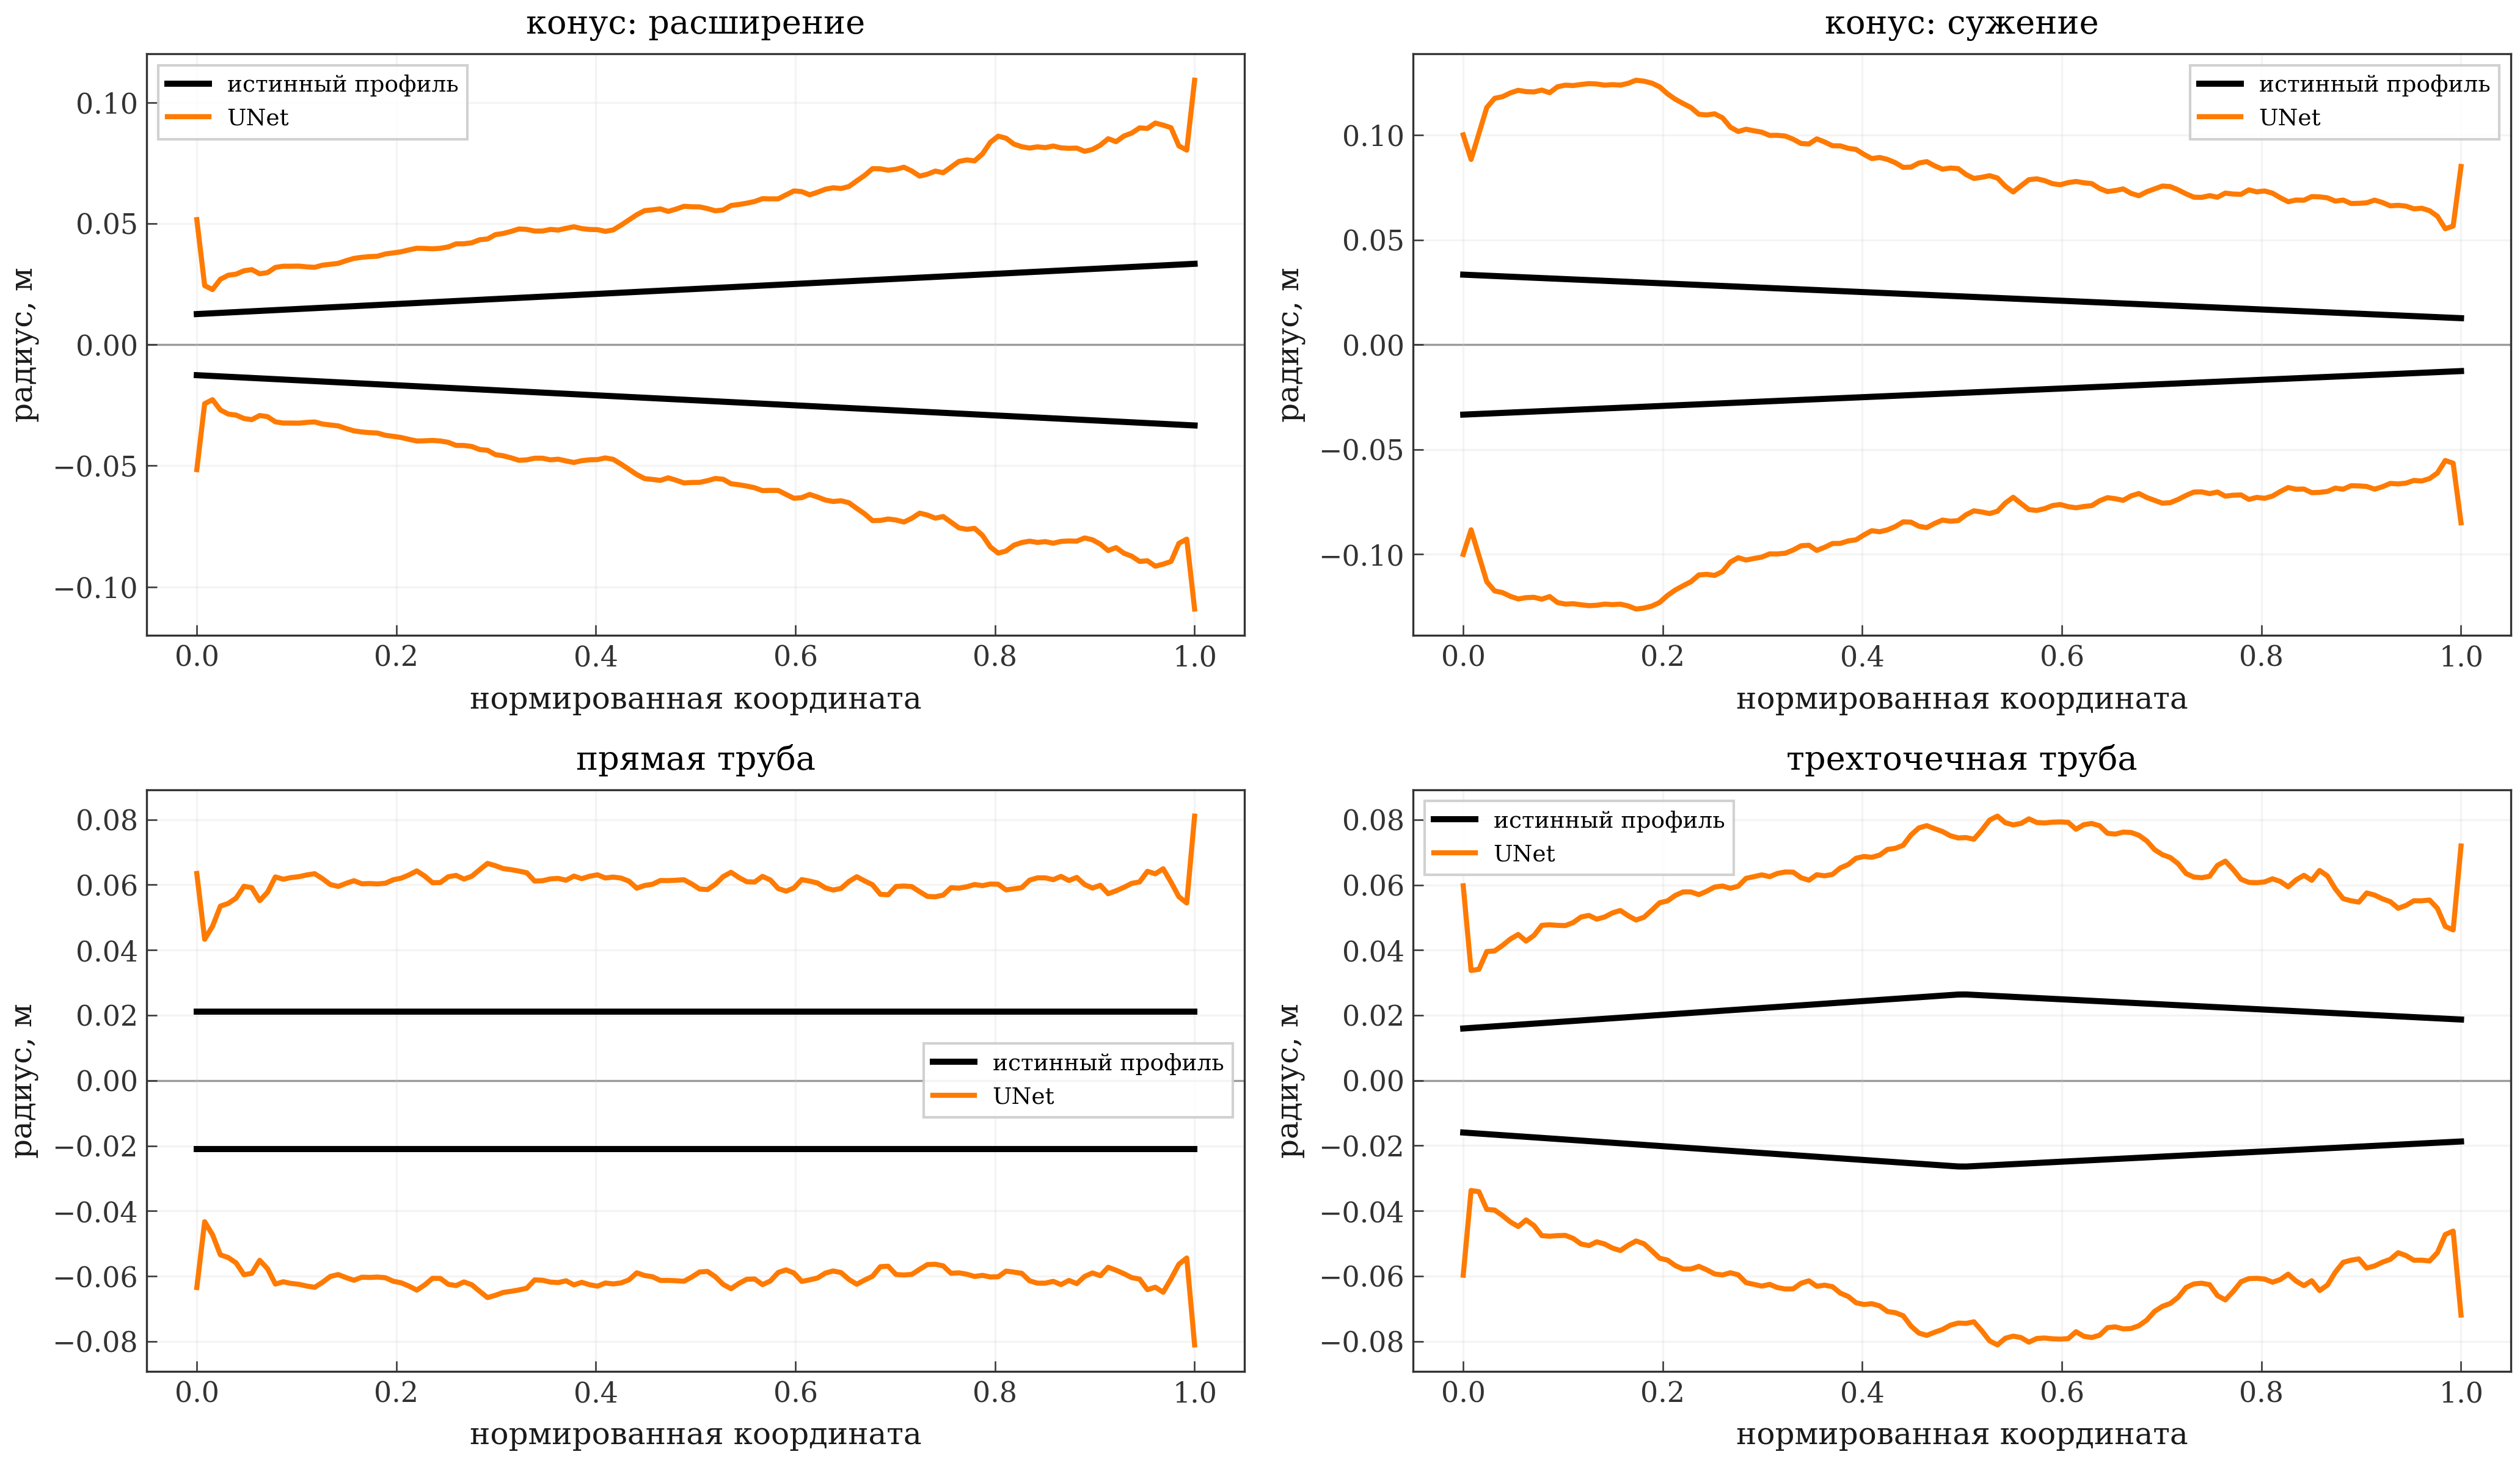
\includegraphics[width=0.95\textwidth]{images/обратная_задача_unet_четыре_геометрии.png}
    \caption{Примеры восстановления геометрических профилей четырех различных тестовых волноводов с помощью обученной сверточной модели UNet.}
    \label{fig:unet_reconstructions}
    \label{fig_count} % Для подсчета рисунков в аннотации
\end{figure}
